%%%%%%%%%%%%%%%%%%%%%%%%%%%%%%%%%%%%%%%%%%%%%%%%%%%%%%%%%%%%%%%%%%%%%%%%%%%%
% grlsample.tex: this sample file is for articles formatted with LaTeX2e,
% Modifiied June 2004
%
% This template is set up logically, with commands and instructions
% given in the order necessary to produce a final output that will
% satisfy AGU requirements.
%
% PLEASE DO NOT USE YOUR OWN MACROS
%
% All questions should be e-mailed to author.help@agu.org.
%%%%%%%%%%%%%%%%%%%%%%%%%%%%%%%%%%%%%%%%%%%%%%%%%%%%%%%%%%%%%%%%%%%%%%%%%%%%
%
%   ARTICLE MODE
%
% PLEASE USE THE GALLEY OPTION TO SUBMIT YOUR PAPERS
% IF YOU HAVE MULTI-LINE EQUATIONS
% The galley option produces single spaced, single column output
%
%LaTeX2e (galley):
\documentclass[galley,ras]{agu2001}
% LaTeX2e (draft):
%\documentclass[draft,grl]{agu2001}
%
%% ------------------------------------------------------------------------ %%
%
%  IMAGE DISPLAY
%
%% ------------------------------------------------------------------------ %%
%
% Uncomment the following line if you need to include images
\usepackage{graphicx}
%
% PLEASE NOTE: WHEN YOU SUBMIT YOUR LATEX FILE TO GEMS, COMMENT OUT ANY COMMANDS
% THAT INCLUDE GRAPHICS.
% (See FIGURES section near the end of the file)

%% ------------------------------------------------------------------------ %%
%
%  ENTER PREAMBLE
%
%% ------------------------------------------------------------------------ %%

\authorrunninghead{OSWALD ET AL.}
% Author names in capital letters,

\titlerunninghead{DETERMINATION OF THE EFFECTIVE LENGTH VECTORS OF THE STEREO ANTENNAS}
% Shorter version of title entered in capital letters

% Author address will appear at end of article, may repeat
% this command for each author.
\authoraddr{T.H. OSWALD,
Space Research Institute, Schmiedlstrasse 6, Graz, A-8042, Austria.
(thomas.oswald@oeaw.ac.at)}


\begin{document}

%% ------------------------------------------------------------------------ %%
%
%  ENABLE IMAGE DISPLAY WHILE USING DRAFT MODE
%
%% ------------------------------------------------------------------------ %%
%
% Uncomment the following code (as well as \usepackage{graphicx} above)
% if you need to include images in draft mode
\setkeys{Gin}{draft=false}
%
% PLEASE NOTE: WHEN YOU SUBMIT YOUR LATEX FILE TO GEMS, COMMENT OUT ANY COMMANDS
% THAT INCLUDE GRAPHICS.
% (See FIGURES section near the end of the file)
%

%% ------------------------------------------------------------------------ %%
%
%  TITLE
%
%% ------------------------------------------------------------------------ %%


\title{The numerical determination of the effective length vectors of the STEREO/SWAVES monopole antennas}
%
% e.g., \title{Terrestrial Ring Current:
% Origin, Formation and Decay $\alpha\beta\Gamma\Delta$}

%% ------------------------------------------------------------------------ %%
%
%  AUTHORS AND AFFILIATIONS - 3 methods
%
%% ------------------------------------------------------------------------ %%


% ---------------
% Method 2 (for all journals, except Reviews of Geophysics, which
% should use method 3):
% For more than three author/affiliation blocks,
% use \author{\altaffilmark{}} and \altaffiltext{}
% \altaffilmark will produce footnote;
% matching altaffiltext will appear at bottom of page.
% May use \\ to start a new line.

 \authors{Oswald, T.H.,\altaffilmark{1}
 H.O. Rucker, \altaffilmark{1}
 W. Macher, \altaffilmark{1}
G. Fischer, \altaffilmark{2}
U. Taubenschuss, \altaffilmark{1}
M.L. Kaiser, \altaffilmark{3}
  K. Goetz,\altaffilmark{4}
 J.L. Bougeret, \altaffilmark{5}
 and  A. Lecacheux\altaffilmark{5} }

 \altaffiltext{1}
 {Space Research Institute, Austrian Academy of Sciences, Graz, Austria.}
%
 \altaffiltext{2}
 {Department of Physics and Astronomy, University of Iowa, Iowa City, USA.}

 \altaffiltext{3}{NASA/GSFC, Greenbelt, MD, USA.}
%
 \altaffiltext{4}{University of Minnesota, USA.}
%
\altaffiltext{5}{Observatoire de Paris-Meudon/ LESIA, France}


%% ------------------------------------------------------------------------ %%
%
%  ABSTRACT
%
%% ------------------------------------------------------------------------ %%

% Do NOT include any \begin...\end commands within
% the body of the abstract.

\begin{abstract}
STEREO is a space mission conducted by NASA, to be launched in April 2006. It consists of two spacecraft which will follow a sun centered trajectory at approximately one AU, one ahead, the other behind earth, slowly drifting apart. The SWAVES experiments onboard the two STEREO spacecraft will perform measurements of the non-thermal radio spectrum from 10 kHz up to about 16 MHz and at 2 frequencies just above 30 MHz. For this purpose 3 orthogonal, six meter long monopole stacer antennas and a set of receivers are used, thereby enabling direction finding, i.e. the determination of the direction of arrival and the polarization state of the observed radio waves. This direction finding capability, which requires an exact knowledge of the antenna properties, in combination with the two spacecraft, opens the possibility to locate the radio sources by means of triangulation. Numerical wire-grid simulations of the antenna system have been performed to determine the effective length vectors of the antennas, which are the most suitable representation of the receiving properties of antennas. The results are presented in this paper and compared with the results of an experimental procedure, with a view to the intended direction finding applications.
\end{abstract}

%% ------------------------------------------------------------------------ %%
%
%  BEGIN ARTICLE
%
%% ------------------------------------------------------------------------ %%

% The body of the article must start with a \begin{article} command,
% and an \end{article} command must be placed at the end of the file,
% before \end{document}.
%
% If using draft mode \end{article} must follow the references section.

\begin{article}

%% ------------------------------------------------------------------------ %%
%
%  TEXT
%
%% ------------------------------------------------------------------------ %%

\section{Introduction}
The existence of two spatially separated spacecraft observing radiation of the same source simultaneously,
 in combination with direction finding capabilities, enables a new type of observation. The location of
  the radio sources can be pinpointed via triangulation and its evolution can be tracked from the surface
 of the sun, to earth's orbit and beyond.\\

Direction finding is the procedure of finding the direction of the incident wave as well as the Stokes parameters,
 which define the state of its polarization, from the measured observables. The measured observables are the auto-
  and cross-correlation parameters of the antennas. For three axes stabilized spacecraft with three antennas,
 like the STEREO spacecraft, there exist equations which can be used to perform this task (\cite{cecconi05}).
  But to succeed, it is of vital importance to know the reception properties of the antennas to a high degree of
   accuracy. A very elegant and concise method of describing the receiving property of an antenna is the effective
  length vector, which is a generalization of the well known effective height. Four known methods exist to determine
 the effective length vector of a spacecraft antenna:\\

\begin{enumerate}
    \item Numerical wire grid modeling\\
\item Experimental rheometry\\
\item The EMC chamber\\
\item In-flight calibration\\
\end{enumerate}

The effective length vectors and impedances of the STEREO/WAVES antennas were computed by a numerical method, using the open source ASAP software and several routines developed by the radio-science group of the space research institute in Graz. In this paper we determine the effective length vectors of the antennas of the STEREO spacecraft, which is, in our opinion, the most suitable representation of the properties of a receiving antenna which is used for direction finding. We discuss the theory, present the results of the numerical calculation and compare them with the results of an experimental method.


%% ------------------------------------------------------------------------ %%
%
%  SECTION HEADS
%
%% ------------------------------------------------------------------------ %%

% Level 1 head

% Use the \section{} command to identify level 1 heads;
% type the appropriate head wording between the curly
% brackets, as shown below.
%
% Capitalize the first letter of each word (expect for
% prepositions, conjunctions, and articles that are
% three or fewer letters).
%
% Do not hyphenate level 1 heads. To break lines,
% type \protect\\ where you want the break to occur.
% AGU prefers the inverted triangle, breaking before
% prepositions, conjunctions, and articles, if possible.



\section{The spacecraft and the SWAVES experiment}
There are two types of antennas used on most spacecraft. One type is used for communication. Normally parabolic antennas are well suited for this task. The other type of antennas to be discussed here, is used to receive radiation from natural sources. Simple antennas, like monopole, dipole or loop antennas are used in this case. The STEREO/WAVES experiment works with three mutually orthogonal stacer monopole antennas. They are connected to several receivers:\\

\begin{itemize}
    \item FFR   fixed frequency receiver\\
\item HFR   high frequency receiver\\
\item LFR   low frequency receiver\\
\item TDS   time domain sampler\\
\item LWS   Langmuir wave statistics\\
\item LSR   low rate science\\
\end{itemize}

The most important receivers from our point of view are the HFR which operates in a range from 125 kHz to 16.025 MHz, the LFR and the FFR which operates at 30.025 MHz and 32.025 MHz.\\

The HFR provides 12 bit data, as compared to the 8 bit data of the CASSINI/RPWS receiver, and will provide all auto and cross correlation parameters (these parameters are explained in the next section). Two direction finding modes are planned, one of which uses the antennas as dipoles, like RPWS did. The other DF mode uses the antennas as monopoles. Each sweep will take approximately 15 seconds. \\

The LFR comprises 3 frequency bands, A, B and C. The ranges are\\

\begin{itemize}
    \item A: 2.5-10 kHz\\
\item B: 10-40 kHz\\
\item C: 40-160 kHz\\
\end{itemize}

Bands B and C can provide auto correlation parameters and be used for DF. The data produced by the LFR also has a accuracy of 12 bits.\\

The FFR operates only at the two frequencies mentioned above. As result of the frequencies, which are considerably higher than the range to be used for DF, a special treatment is required. The use of the effective length vectors as a tool for representing the antenna properties seems not appropriate at these frequencies. Therefore we calculate and present the radiation patterns instead.\\

The base capacitances of antennas, coax cables and receivers, we were estimated to be 90pF.\\

\section{The effective length vector as representation of the transmitting and receiving antenna}
A highly useful concept which will be used extensively in this article is the effective length vector. It can be defined as a vector such that the equation


\begin{equation}
 V=\textbf{h}_{eff}\cdot \textbf{E}
 \end{equation}

is satisfied for a monochromatic electromagnetic wave. V is the voltage at the feed. Providing the reciprocity theorem is valid, one can also use the concept for receiving antennas such that the induced voltage can be calculated if the effective length vector and the magnitude, direction and polarization of the incident wave are known.\\

Hence, the effective length vector comprises the complete information of the shape of the antenna. Due to the fact that the skin of a spacecraft is normally conducting, in acts as part of the antenna itself. The usefulness of the concept of the effective length vector can be understood by realizing that the complicated shape of the spacecraft hull can be condensed into a single vector in the context of antenna properties. The effective length vector can be calculated by the following integral:

\begin{equation}
\textbf{h}_{eff}=\frac{1}{I}\int \mathbf{J}(\mathbf{r}')e^{\imath \mathbf{k} \cdot \mathbf{r}'} dV
 \end{equation}

In general it is complex and depends upon direction of the incident wave. These dependencies can safely be neglected at low frequencies, where the effective length vector can be regarded as real and constant. This range is called the quasistatic range. In this frequency range, most known direction finding techniques work with satisfying accuracy. It is of vital importance to know the upper boundary of this range. For the STEREO/SWAVES antennas the boundary can be estimated to be approximately 2 MHz as described later.\\

The magnitude and direction of the effective length vectors are parameters of the usual direction finding methods (see \cite{cecconi05} for instance). The relation between the vector potential in the far field and the effective length vector is

\begin{equation}
% \nonumber to remove numbering (before each equation)
  \mathbf{A} = \frac{\mu_0 I \textbf{h}_{eff}}{4 \pi r}e^{-\imath k r}
\end{equation}

On base of the vector potential all other fields of the transmitting antenna can be computer with the standard equations.\\

At high frequencies, where the wavelength of the incident wave can not be regarded as large in relation to the spacecraft dimensions, the effective lengths vector depends on frequency and direction of the radiation and the imaginary part becomes large. Special care has to be taken when the effective length vectors are used in this range.


\section{Antennas on spacecraft, the Stokes parameters and the effective length vectors}

The auto- and cross-correlation parameters for two antennas, say i and j, are defined as the average product of the voltage induced on one antenna with the complex conjugate of the voltage induced on the same, or the other antenna, respectively. So for two antennas i and j they are

\begin{eqnarray}
% \nonumber to remove numbering (before each equation)
  \left\langle V_i V_i^* \right\rangle  \nonumber \\
 \left\langle V_i V_i^* \right\rangle  \nonumber \\
 \Re \left\langle V_i V_j^* \right\rangle  \nonumber \\
 \Im \left\langle V_i V_j^* \right\rangle \nonumber
\end{eqnarray}

and the time average can be understood as

\begin{equation}
 \left\langle CC^* \right\rangle = \frac{1}{T}\int_0^T CC^* dt
 \end{equation}

where the integration time T must be long in relation to the period of the received radiation.\\

The Stokes parameters $S_0$ to $S_3$ are one of several possibilities of representing the state of polarization of the received wave. The normalized parameters $\hat{I}$, $\hat{Q}$, $\hat{U}$ and $\hat{V}$ can be written as


\begin{eqnarray} \frac{S_0}{2\eta_0} = \hat{I} &=& \frac{\left\langle E_{x}^2\right\rangle +\left\langle E_{y}^2\right\rangle}{2\eta_0} \label{norm_stokes_1} \\
\frac{S_1}{S_0}=\hat{Q}&=&\frac{\left\langle E_{x}^2\right\rangle-\left\langle E_{y}^2\right\rangle}{\left\langle E_{x}^2\right\rangle +\left\langle E_{y}^2\right\rangle}\label{norm_stokes_2} \\ \frac{S_2}{S_0}=\hat{U}&=&\frac{\left\langle2E_{x} E_{y} \cos\delta\right\rangle}{\left\langle E_{x}^2\right\rangle +\left\langle E_{y}^2\right\rangle}
\label{norm_stokes_3} \\
\frac{S_3}{S_0}=\hat{V}&=&\frac{\left\langle2E_{x} E_{y} \sin\delta\right\rangle}{\left\langle E_{x}^2\right\rangle +\left\langle E_{y}^2\right\rangle}\label{norm_stokes_4}
\end{eqnarray}

where $E_{x}$ and $E_{y}$ are the components of the electric field in the direction of the x- and y-axes of the wave frame, given that the wave vector \textbf{k} points along the z-axis. $\eta_0$ is the impedance of free space and $\delta $ the phase shift between the components of the electric field in the x and y direction.\\



\section{Direction finding}\label{sec_DF}
When the coordinate frame shown in figure \ref{fig_coord_frame} is used, the following relationship between the correlation parameters for antennas i and j on one side and the coordinates and Stokes parameters on the other side can be found (see \cite{my_masterthesis}):


\begin{eqnarray}
\left\langle V_i V_i^{*} \right\rangle &=& \hat{S}\eta_0 h_{eff,i}^2[(\hat{Q}+1) (\sin^2 \theta \cos^2 \alpha_i -\nonumber\\
& & -\frac{1}{2} \sin (2\alpha_i) \sin(2\theta) \cos^2(\varphi - \Omega_i) + \nonumber \\
& & + \sin^2\alpha_i \cos^2\theta \cos^2(\varphi - \Omega_i))+ \nonumber \\
& & + (1-\hat{Q}) \sin^2\alpha_i \sin^2 (\varphi - \Omega_i)+ \nonumber \\
& & +  \hat{U}  (-\sin \theta \sin 2\alpha_i \sin(\varphi - \Omega_i) +\nonumber \\
& & + \sin^2\alpha_i \cos \theta sin(2\varphi - 2\Omega_i)) ]
\end{eqnarray}

\begin{eqnarray}
\Re \left\langle V_i V_j^{*}\right\rangle &=& \hat{S}\eta_0 h_{eff,i} h_{eff,j}[(\hat{Q}+1) (\sin^2 \theta \cos \alpha_i \cos \alpha_j - \nonumber\\
& & - \frac{1}{2}  \sin(2\theta) (\sin \alpha_j \cos \alpha_i \cos(\varphi - \Omega_j)+\nonumber \\
& & +\sin \alpha_i \cos \alpha_j \cos(\varphi - \Omega_i) ) + \nonumber \\
& & + \sin \alpha_i \sin \alpha_j \cos^2\theta \cos(\varphi - \Omega_i) \cos(\varphi - \Omega_j))+ \nonumber \\
& & + (1-\hat{Q}) \sin \alpha_i \sin \alpha_j \sin (\varphi - \Omega_i) \sin (\varphi - \Omega_j)-\nonumber \\
& & -\hat{U} (\sin \theta(\sin \alpha_i \cos \alpha_j \sin (\varphi - \Omega_i) +  \nonumber \\
& & + \sin \alpha_j \cos \alpha_i \sin (\varphi - \Omega_j))- \nonumber \\
& & - \cos \theta \sin \alpha_i \sin \alpha_j(\sin (\varphi - \Omega_j) \cos (\varphi - \Omega_i)+ \nonumber \\
& & + \sin (\varphi - \Omega_i) \cos (\varphi - \Omega_j) ) )]
\end{eqnarray}

\begin{eqnarray}
\Im \left\langle V_i V_j^{*}\right\rangle &=& - \hat{S}\eta_0 h_{eff,i} h_{eff,j} \hat{V}[ \sin \theta(\sin \alpha_i \cos \alpha_j \sin (\varphi - \Omega_i) - \nonumber\\
& & - \sin \alpha_j \cos \alpha_i \sin (\varphi - \Omega_j))+ \nonumber \\
& & +\cos \theta \sin \alpha_i \sin \alpha_j(\sin (\varphi - \Omega_j) \cos (\varphi - \Omega_i)+ \nonumber \\
& & + \sin (\varphi - \Omega_i) \cos (\varphi - \Omega_j) ) ]
\end{eqnarray}

$h_{eff,i}$ and  $h_{eff,j}$ are the magnitudes of the effective length vectors of antennas i and j, respectively, $\alpha$ and $\Omega$ are the polar angles describing the direction of the respective antenna, while $\theta$ and $\phi$ are the polar angles describing the direction of the incident wave. Since all three antennas can be combined at the SWAVES experiment, there are 9 equations for 6 unknown parameters. When the coordinate frame is chosen in a way that the effective length vector of one antenna points in the direction of one coordinate axis, say the Z antenna along the Z-axis, an analytical solution for the direction of the incident wave can be found.


\begin{eqnarray}\label{tan_phi}
\tan \varphi &=& [\Im \left\langle V_X V_Z^{*}\right\rangle h_{eff,Y} \sin \alpha_Y \tan \Omega_Y \cos \Omega_Y-\nonumber\\
& & -\Im \left\langle V_Y V_Z^{*}\right\rangle h_{eff,X} \sin \alpha_X \tan \Omega_X \cos \Omega_X] \times \nonumber \\ & &\times[\Im \left\langle V_X V_Z^{*}\right\rangle h_{eff,Y} \sin \alpha_Y \cos \Omega_Y -\nonumber \\
& &  -\Im \left\langle V_Y V_Z^{*}\right\rangle h_{eff,X} \sin \alpha_X  \cos \Omega_X]^{-1}
\end{eqnarray}


\begin{eqnarray}\label{tan_theta}
\tan \theta\  &=& [\left\langle V_Z V_Z^{*} \right\rangle h_{eff,X} h_{eff,Y} \sin \alpha_X  \sin \alpha_Y \nonumber \\
&&\times ( \cos (\varphi - \Omega_Y)  \sin (\varphi - \Omega_X) -\nonumber \\
&&-\cos (\varphi - \Omega_X)  \sin (\varphi - \Omega_Y))]\nonumber \\
&& \times [\Re \left\langle V_X V_Z^{*}\right\rangle \sin \alpha_Y  \sin (\varphi - \Omega_Y) h_{eff,Y}h_{eff,Z} \nonumber \\
&&-\Re \left\langle V_Y V_Z^{*}\right\rangle\sin \alpha_X  \sin (\varphi - \Omega_X) h_{eff,X}h_{eff,Z}\nonumber \\ &&+\left\langle V_Z V_Z^{*} \right\rangle h_{eff,X} h_{eff,Y} \nonumber \\
&&\times(\cos \alpha_Y \sin \alpha_X  \sin (\varphi - \Omega_X)-\nonumber \\
&& -\cos \alpha_X  \sin \alpha_Y  \sin (\varphi - \Omega_Y))]^{-1}
\end{eqnarray}

A detailed derivation can be found in (\cite{my_masterthesis}). See also \cite{cecconi05} for the derivation of a similar equation with a slightly different coordinate frame. The solution for $\varphi$ is not unambiguous, as one has to know the half sphere of the radio source in advance. It should be emphasized that not all available observables are used in these solutions, which results in loss of information. There exist numerical methods where this is avoided. For a general treatment of these possible methods see (\cite{my_masterthesis}). To compute the Stokes parameters once the direction is known, the method published in (\cite{cecconi05}) can be used. A matrix equation is formed, which can be solved analytically. The equation, suitable for our coordinate frame is\\

\begin{equation}\label{lineare_gleichung}
\textbf{M}\textbf{x}=\textbf{b}
\end{equation}

with\\

\begin{equation}
\textbf{b}=\left[ \begin{array}{c} \frac{\left\langle V_X V_X^{*} \right\rangle }{\eta_0 h_{eff,X}^2} \\
\\
\frac{\left\langle V_Z V_Z^{*} \right\rangle }{\eta_0 h_{eff,Z}^2}\\
\\
\frac{\Re \left\langle V_X V_Z^{*}\right\rangle }{\eta_0 h_{eff,X} h_{eff,Z}} \\
\\
\frac{\Im \left\langle V_X V_Z^{*}\right\rangle }{\eta_0 h_{eff,X} h_{eff,Z}}\end{array}
\right]
\end{equation}

\begin{equation} \textbf{x}=\left[ \begin{array}{c} \hat{S}\\ \hat{S}\hat{Q}\\
\hat{S}\hat{U}\\
\hat{S}\hat{V} \end{array}  \right]
\end{equation}


\begin{equation} \textbf{M}= \left[ \begin{array}{cccc} M_{11} & M_{12} & M_{13} & 0 \\
M_{21} &M_{22}  & M_{23} & 0 \\
M_{31}& M_{32} & M_{33} & 0 \\
0 & 0 & 0 &M_{44}
\end{array} \right]
\end{equation}

where

\begin{eqnarray}
% \nonumber to remove numbering (before each equation)
  M_{11} &=& A^2_X+ B^2_X \\
M_{21} &=& A^2_Z+ B^2_Z \\
M_{31} &=& A_X A_Z +  B_X B_Z \\
M_{12} &=& A^2_X- B^2_X \\
M_{22} &=& A^2_Z- B^2_Z \\
M_{32} &=& A_X A_Z - B_X B_Z \\
M_{13} &=& 2 A_X B_X \\
M_{23} &=& 2 A_Z B_Z \\
M_{33} &=& A_X B_Z + A_Z B_X \\
M_{44} &=& -(-A_X B_Z + A_Z B_X )\end{eqnarray}

and

\begin{eqnarray}
A_i &=& \cos \alpha_i \sin \theta - \sin \alpha_i \cos \theta \cos (\varphi - \Omega_i)\label{A_i} \\
B_i &=& -\sin \alpha_i \sin (\varphi - \Omega_i) \label{B_i}
\end{eqnarray}


Equation (\ref{lineare_gleichung}) is easily solvable, as long as \textbf{M} is not singular. This procedure has been successfully tested, using RPWS data from the Cassini spacecraft. The important aspects of error analysis have been discussed on a theoretical base in (\cite{my_masterthesis}), as well as (\cite{DF}).\\

\section{The numerical method to compute the effective length vectors}
\subsection{Calculation of the current distribution}
The calculation  has to be done in two steps. First the current distribution is computed by using the Method of Moments (MOM). Then, in a second step the effective length vectors are calculated.\\


The calculation of the current distribution on the surface of the spacecraft was done by using a modified version of the Antenna Scatterers Analysis Program (ASAP) which is an open source electromagnetic code. The surface of the spacecraft and the antennas were modeled as a wire grid which is excited by an electromotive force of 1V at the feeds of the antennas. So the electric field integral equations (EFIE) can be used to calculate the currents along the wires, which is a good approximation to the actual current distribution on the real spacecraft if the modeling is done properly.\\

\begin{equation}\label{EFIE}
    \mathbf{E}(\mathrm{r}) = -\frac{\imath \eta}{4 \pi k} \int_S G(\mathbf{r},\mathbf{r}') \mathbf{J}_s (\mathbf{r}') dS'
\end{equation}


$\mathbf{J}_S$ is the surface current density, $G(\mathbf{r},\mathbf{r}')$ is the Green function, $\eta$ is the impedance of free space and k is the wave number. The surface integral over the surface of the spacecraft can be used because the whole spacecraft surface is made of conducting material.\\

This integral equation has to be solved in conjunction with the well known boundary conditions. The integral can be reduced to a scalar integral for the case of a cylindrical wire. Additionally the transverse currents on the wire are ignored and the currents are represented by single filaments along the wire axes. So the boundary conditions have to be satisfied only in axial direction.\\

The integral can be solved numerically by using the MOM which can be found in (\cite{harrington}). It is converted into a matrix equation which can be solved numerically. Hereby the currents along each wire are represented as the sum of a set of two weighed sinusoidal base functions.\\

Once the current distribution is known, the input impedance can be computed by dividing the voltage at the feed by the current.


\subsection{Calculations of the effective length vectors}
The next step is the calculation of the effective length vectors. This can easily be achieved by integrating the retarded surface current density over the whole spacecraft and dividing it by the current at the antenna feed.

\begin{equation}\label{get_heff}
    \mathbf{h}_{eff} = \frac{1}{I_0} \int_S \mathbf{J}_s (\mathbf{r}') e^{- \imath \mathbf{k} \cdot \mathbf{r}}dS'
\end{equation}

$I_0$ is the current at the feed. Details can be found in (\cite{macher_dipl}).

\section{The results of the determination of the effective length vectors of the STEREO/WAVES antennas}
\subsection{Introduction}
Numerical calculations, using ASAP and the ASAP toolbox, to determine the characteristics of the three antennas of the STEREO/SWAVES experiment were performed. Such calculations were done fore the Cassini spacecraft (\cite{cassini}, \cite{cassini2} and \cite{vogl_01}) as well as Mars Express (\cite{marsis} and \cite{marsis2}) and other spacecraft in the past. A summary can be found in (\cite{ruckerundi05}).\\

\subsection{The spacecraft characteristics}

One characteristic of the STEREO spacecraft is a certain degree of asymmetry. In contrast to many other spacecraft, the solar panels are positioned at different longitudinal distances at the spacecraft hull. Additionally the spacecraft consist of an about 6 meters long boom, and a turnable high gain antenna. These prominent features will have an influence on the antenna characteristics. The boom is divided into 4 sections with different diameters and has great influence upon the effective length vectors of the antennas.\\

The used, spacecraft fixed, reference frame is defined in a way to be spacecraft fixed with the positive x-axis in a direction which will point to the sun during most of the time, so the antennas are mounted on the side of the hull which points to the negative x-axis. The solar panels point to the positive and negative y- axis and the z-axis is defined to complete the right handed cartesian frame (see figure \ref{fig_coord_frame}).\\

For the description of the direction of the antennas we chose to use a spherical polar system which has the positive X-axis as polar axis. The angle $\zeta$ is the angle between the positive X-axis and the antenna, and $\xi$ is the azimuthal angle around the X-axis, where antenna E1 is defined to have $\xi=0$.\\

The direction of the boom defines the negative x-axis. There are 3 orthogonal monopole antennas, which are called E1, E2 and E3, each 6 meters long. They are directed about $125.26^\circ$ from the x-axis and the difference in azimuth is $120^\circ$. The azimuth of antenna E1 defines the azimuth of $0^\circ$. It is expected, that the boom has an effect to push the 3 electrical antennas away from the boom's position. This effect is increased by the high gain antenna, which is located near the boom. The panels are expected to push the effective length vectors towards the negative x-axis. \\

The antennas will be directed away from the sun, so that they remain out of view of the sunward looking instruments on the spacecraft. Thus, the most interesting direction of incident waves is the positive x-axis. \\

The two spacecraft, A and B are almost identical, apart of some small differences of their instrumentation. The only difference which can be modeled within the limitations of ASAP is the second ring, mounted on the hull of spacecraft B on the positive x side, and not existent on spacecraft A.\\

With information about the base capacitances of antennas, coax cables and receivers, we were able to estimate and include the total base capacitances to be 90pF.\\


\subsubsection{The model}
The model of the Stereo spacecraft consist of the following parts:\\

\begin{enumerate}
\item The hull
\item 2 solar panels
\item The high gain antenna
\item Three 6 meter long antennas
\item A 6 meter long boom
\item A ring mounted on the hull of spacecraft A, two rings on spacecraft B\\
\end{enumerate}

Size and position of the parts were measured from the relevant construction plans. The part of the tapered boom which is near to the spacecraft hull is modeled as prism with triangular base. Figures \ref{fig_D2_A_Oblique} shows the model from an oblique view. \\
%
\subsection{The Computation}
\subsubsection{Computation of the effective length vectors}
As a first step, we computed the currents at frequencies from 100 kHz to 16 MHz, with a spacing of 100 kHz, each frequency with 19 different angles of the HGA dish. This computation was performed by the ASAP program. Using this data, the impedances, admittances and effective length vectors can easily be computed with the toolbox devised at the Space Research Institute and updated to be suitable for the specific task of analyzing the antennas of SWAVES.\\

\subsection{Calculations}
Figure \ref{fig_Heff_D2_A_Z_ViewCap} shows a plot of the effective length vectors of spacecraft A, in relation to the physical antennas, which are represented in black. The frequency used for these plots is 500kHz, being well in the quasistatic regime. The direction of the incident wave is from the positive x-axis, simulating radiation from the sun.\\

Table \ref{tab_heff} shows the results for all antennas on both spacecraft in tabulated form. The calculations were done for a frequency of 500 kHz and a HGA angle of 0 degrees. For comparison, the lengths and orientation information of the physical antennas are also added.\\

The quasistatic results were in full concurrence with our expectations. All electric antennas have lengths which are shorter than half the length of the physical antennas, as expected by theory for monopole antennas that are small in relation to the wavelength. The influence of the capacitances on the effective length vectors seems to be quite substantial. A similar calculation without taking the capacitances into account resulted in effective length vectors which were approximately half the length of the physical antennas. Furthermore, it can clearly be seen that the solar panels push the electric antennas towards the negative x-axis with a counteracting influence of the boom. The difference between the two spacecraft, although not large, is definitely existent. It should be mentioned, however, that the radii of the antennas of the real spacecraft is not the same as the wire radius used for the calculations. This is a result of the limitations of the ASAP program. There could be a slight change of the magnitude of the effective length vectors due to this different radius. Further research on this matter will be done in future, mainly by using a different code for the current calculation, which allows different wire radii for different parts of the spacecraft.\\

\subsubsection{Variation of the effective length vectors with frequency and direction}

As mentioned before, direction finding is only possible in the lower frequency regions. At higher frequencies, the effective length vectors become complex and dependent on frequency and direction of incidence. The variability of the real part of the effective length vectors can be easily seen on figure \ref{fig_heff_dist_D2_A_Z_View_caps}. The plot was constructed by choosing 26 different directions and computing the effective length vectors for each frequency and each direction. The real part of all effective length vectors were plotted. The frequency is color coded. The imaginary parts of the vectors were ignored. The 26 sample directions were chosen to be the corners of a cube, and the midpoints of each area and each edge. The reason for the erratic behavior at high frequencies is the resonance at 14 MHz. Even though only the figures for spacecraft A are included, the plots of the antennas of spacecraft B show comparable results.\\


When direction finding is regarded to be possible with the knowledge of the directions of the electric antennas with an accuracy of 2 degrees, further analysis dictate an upper limit of not more than 2MHz where direction finding can be done by using standard methods. Fortunately further analysis shows that, even in the region near the resonance frequency, the effective length vectors behave in a predictable manner, i.e. they are not chaotic. Figure \ref{fig_heff_dist_6d_500kHz_caps} shows the distance of the tip of the effective length vector of the E1 antenna from the quasistatic effective length vector in three dimensional complex space as a function of direction of incidence at a frequency of 500 kHz.. It clearly can be seen that the function is continuous. The same is true for figure \ref{fig_heff_dist_6d_13.5MHz_caps}, although the variations are larger. This figure shows the result at 13.5 MHz, which is very near to the first resonance frequency. Further analysis shows that the function is also continuous regarding frequency variations.\\


\subsubsection{Variation of the effective length vectors with frequency at fixed direction}
The radiation to be measured by the spacecraft will have a direction of arrival roughly from the sun, which is located opposite to the boom (positive x-axis). Therefore it is useful to compute the geometry of the effective length vectors for this direction in detail. Figures \ref{fig_Heff_length_real_caps_D2} and \ref{fig_Heff_length_imag_caps_D2} show the length of the effective length vectors as a function of frequency. Again, the result for STEREO A is plotted in solid lines while the results for STEREO B is plotted in dashed lines.\\

As one can see, the resonances at 14MHz change drastically the effective lengths of the antennas. The imaginary part of $\mathbf{h_{eff}}$ vanishes as the frequency goes to zero while the real part converges to the quasistatic limit.\\

\subsubsection{Variation of the effective length vectors with different HGA angles}
Analysis of the influence of the orientation of the HGA upon the effective length vectors has shown that the deviation is, in general, less then one degree at low frequencies. As an example, the coordinates of the effective length vector of E1 is shown in table \ref{tab_e1_var}. The frequency used to produce this data was 500kHz. \\


\subsubsection{The impedances and admittances}
On the plots of the admittances, the first resonances can be seen at a frequency between 13 and 14 MHz. A resonance exists, if the effective length of the antenna is equal to $\frac{1}{4}$ of the wavelength of the incident radiation. In the case of the spacecraft, the length of the distance between the tip of the antenna and the furthest point on the spacecraft represents half of the wavelength. In case of STEREO, the longest distances are between the boom and the antennas and between the edge of the opposite solar panel and the tip of the antennas. The wavelength of an electromagnetic wave at 12 MHz is 25 meters, so $\frac{\lambda}{4}$ is 6.25 m. Hence we would expect two resonances in the frequency range around 12MHz, but the inclusion of the capacitances of the receiver, the cable and the antenna mounting has the effect to decrease the resonance frequency. When regarding the case of transmitting antennas, the base capacitances are parallel to the antenna capacitances and both can be added. To get the overall impedance, the reciprocal values have to be added, while the admittances have simply to be added. The two resonances can partly be seen on the plot of the admittances, but in general they are too close together to be resolved. \\

One example of the resultant impedance can be seen in Figures \ref{fig_Impedance1_D2_caps} and \ref{fig_Impedance2_D2_caps}. While in the first plot, the real and imaginary parts are plotted as a function of frequency, the imaginary part is plotted as a function of the real part in the lower graph. The resonance occurs when the imaginary part of the impedance is zero. Then the antenna is pure resistive. It can clearly be seen in the plots.
%

\section{Conclusion}
The NASA mission STEREO will provide new insights into the physics of the solar system by using stereoscopic methods to analyze radio sources. It has been shown that the method relies on direction finding, of which a short overview was given in section \ref{sec_DF}. It was also shown that direction finding relies heavily upon a detailed knowledge of the receiving properties of the antennas, which can be represented by a single entity, the effective length vector. A numerical method was used to compute the effective length vectors of the antennas of the STEREO spacecraft. \\
%
%% ------------------------------------------------------------------------ %%

% Do not use bulleted lists; enumerated lists are okay.
% begin{enumerate}
% \item
% \item
% \item
% \end{enumerate}

%% ------------------------------------------------------------------------ %%
%
%  EQUATIONS
%
%% ------------------------------------------------------------------------ %%

% Single-line equations are centered.

% Math coded inside display math mode $$...$$
% will not be numbered e.g.:
%$$x^2=y^2 + z^2$$

% Math coded inside \begin{equation} and \end{equation} will
% be automatically numbered e.g.:
 %\begin{equation}
 %x^2=y^2 + z^2
 %\end{equation}

% IF YOU HAVE MULTI-LINE EQUATIONS, PLEASE
% BREAK THE EQUATIONS INTO TWO OR MORE LINES
% OF SINGLE COLUMN WIDTH (20 pc, 8.3 cm)
% using double backslashes (\\).

% To create multiline equations, use the
% \begin{eqnarray} and \end{eqnarray} environment
% as demonstrated below.
%\begin{eqnarray}
%  x_{1} & = & (x - x_{0}) \cos \Theta \nonumber \\
%        && + (y - y_{0}) \sin \Theta  \nonumber \\
%  y_{1} & = & -(x - x_{0}) \sin \Theta \nonumber \\
%        && + (y - y_{0}) \cos \Theta.
%\end{eqnarray}


% Break each line at a sign of operation
% (+, -, etc.) if possible, with the sign of operation
% on the new line.

% Indent second and subsequent lines to align with
% the first character following the equal sign on the
% first line.

% Use an \hspace{} command to insert horizontal space
% into your equation if necessary. Place an appropriate
% unit of measure between the curly braces, e.g.
% \hspace{1in}; you may have to experiment to achieve
% the correct amount of space.

% There is another multiline equation environment:
% \begin{aguleftmath}...\end{aguleftmath}
% The equation is aligned left and the second line indents to
% the width of a paragraph indent (AGU style)


%% ------------------------------------------------------------------------ %%
%
%  EQUATION NUMBERING: COUNTER
%
%% ------------------------------------------------------------------------ %%

% You may change equation numbering by resetting
% the equation counter or by explicitly numbering
% an equation.

% To explicitly number an equation, type \eqnum{}
% (with the desired number between the brackets)
% after the \begin{equation} or \begin{eqnarray}
% command.  The \eqnum{} command will affect only
% the equation it appears with; LaTeX will number
% any equations appearing later in the manuscript
% according to the equation counter.
%
% To reset the equation counter, place the setcounter{equation}
% command in front of your equation(s).
%\setcounter{equation}{0}

% Set the equation counter to 0 if the next
% number needed is 1 or set it to 7 if the
% next number needed is 8, etc.
%
% The \setcounter{equation} command does affect
% equations appearing later in the manuscript.

% If you have a multiline equation that needs only
% one equation number, use a \nonumber command in
% front of the double backslashes (\\) as shown in
% the multiline equation above.





%% ------------------------------------------------------------------------ %%
%
%  ACKNOWLEDGMENTS
%
%% ------------------------------------------------------------------------ %%

\begin{acknowledgments}
I thank Prof. Rucker for letting me participate in this interesting branch of research, as well as for the support he gave me. I also thank my colleagues for their valuable contributions to this work.
\end{acknowledgments}

%% ------------------------------------------------------------------------ %%
%
%  REFERENCE LIST AND TEXT CITATIONS
%
%% ------------------------------------------------------------------------ %%
%
% If you use BiBTeX for your References, please do not send
% your bibliography database. Copy the reference list
% from your .bbl file into your article file before submission:
%
%1. Run LaTeX on your LaTeX file.
%
%2. Run BiBTeX on your LaTeX file.
%
%3. Open the new .bbl file containing the reference list and
%copy all the contents into your LaTeX file after the
%acknowledgments section;
%
%4. Comment out the old \bibliographystyle and \bibliography commands.
%
%5. Run LaTeX on your new file before submitting.

%Failure to follow these instructions will require manual
%intervention through hard keying of information,
%which can introduce errors.

\begin{thebibliography}{}

\providecommand{\natexlab}[1]{#1} \expandafter\ifx\csname urlstyle\endcsname\relax  \providecommand{\doi}[1]{doi:\discretionary{}{}{}#1}\else  \providecommand{\doi}{doi:\discretionary{}{}{}\begingroup  \urlstyle{rm}\Url}\fi


\bibitem[{\textit{Cecconi and Zarka}(2005)}]{cecconi05} Cecconi, B., and P.~Zarka (2005), Direction finding and antenna calibration  through analytical inversion of radio measurements performed using a system  of 2 or 3 electric dipole wire antennas on a 3 axes stabelized spacecraft,  \textit{ Radio Sci.}, \textit{40}, RS3003, doi:10.1029/2004RS003070.



\bibitem[{\textit{Fischer et~al.}(2001)}]{cassini} Fischer, G., W.~Macher, H.~Rucker, H.~Ladreiter, and D.~Vogl (2001), Wire-grid  modeling of Cassini spacecraft for the determination of effective antenna  length vectors of the RPWS antennas, in \textit{Proc. Planetary Radio  Emissions V}, edited by H.~Rucker, M.~Kaiser, and Y.~Leblanc, pp. 347--356,  Austrian Academy of Sciences Press, Vienna.

\bibitem[{\textit{Fischer et~al.}(2003)}]{cassini2} Fischer, G., W.~Macher, H.~Rucker, H.~Ladreiter, and D.~Vogl (2003), Reception  properties of the Cassini/RPWS antennas from 1 to 16 mhz, poster at the  EGS-AGU-EUG Joint Assembly, Nice.


\bibitem[{\textit{Harrington}(1968)}]{harrington}
Harrington, R. (1968), \textit{Field Computation by Moment Methods}, Robert E.
  Krieger Publishing Company.

\bibitem[{\textit{Macher}(1997)}]{macher_dipl} Macher, W. (1997), Theorie effektiver hoehenvektoren von antennen mit anwendung  auf das radio and plasma wave science experiment der Cassini raumsonde,  Diploma thesis, Graz University of Technology.

\bibitem[{\textit{Macher et~al.}(2002)}]{marsis} Macher, W., B.~Schrausser, G.~Fischer, H.~Rucker, H.~Lammer, C.~Kolb, and  G.~Kargl (2002), Analysis of sounding antennas of the mars-express marsis  experiment, in \textit{Proc. 2nd European Workshop on Exo/Astrobiology},  edited by H.~Sawaya-Lacoste, pp. 539--540, ESA Publications Division,  Noordwijk, ESA SP-518.

\bibitem[{\textit{Macher et~al.}(2004)}]{marsis2} Macher, W., H.~Rucker, G.~Fischer, and M.~Team (2004), Analysis of the marsis  antenna system onboard mars express, poster at the EGU 1st General Assembly,  Nice.

\bibitem[{\textit{Oswald}(2005)}]{my_masterthesis}
Oswald, T.H. (2005), Electromagnetic waves in space and the stereo/waves
  experiment, Master's thesis, University of Graz.


\bibitem[{\textit{Oswald et~al.}(2005)}]{DF} Oswald, T., H.~Rucker, W.~Macher, G.Fischer, and U.~Taubenschuss  (2005{\natexlab{b}}), Direction finding, \textit{Technical Report of the  Space Research Institute/Austrian Academy of Science}, \textit{Nr. 168}.

\bibitem[{\textit{Rucker et~al.}(1997)}]{cassini3} Rucker, H.~O., W.~Macher, and S.~Albrecht (1997), Experimental and theoretical  investigations on the Cassini RPWS antennas, in \textit{Proc. Planetary Radio  Emissions IV}, edited by H.~Rucker, S.~J. Bauer, and A.~Lecacheux, pp.  327--337, Austrian Academy of Sciences Press Vienna.

\bibitem[{\textit{Rucker et~al.}(2005)}]{ruckerundi05} Rucker, H., W.~Macher, G.~Fischer, T.~Oswald, J.-L. Bougeret, M.~Kaiser, and  K.~Goetz (2005), Analysis of spacecraft antenna systems: Implications for  stereo/waves, \textit{Adv. Space Res.},\textit{36},1530-1533, \doi{10.1016/j.asr.2005.07.060}.



\bibitem[{\textit{Vogl et~al.}(2001)}]{vogl_01} Vogl, D., H.~Ladreiter, P.~Zarka, H.~Rucker, W.~Macher, W.~S. Kurth,  D.~Gurnett, and G.~Fischer (2001), First results on the calibration of the  Cassini RPWS antenna system., in \textit{Proc. Planetary Radio Emissions V},  edited by H.~Rucker, M.~Kaiser, and Y.~Leblanc, pp. 357--366, Austrian  Academy of Sciences Press, Vienna.

\bibitem[{\textit{Vogl et~al.}(2004)}]{vogl_04} Vogl, D., et~al. (2004), In-flight calibration of the Cassini/RPWS antenna  system for direction finding and polarization measurements, \textit{J.  Geophys. Res.}, \textit{109}, A09S17, \doi{10.1029/2003JA010261}.
\end{thebibliography}

%% ------------------------------------------------------------------------ %%
%
% FIGURES
%
% PLEASE NOTE: WHEN YOU SUBMIT YOUR LATEX FILE TO GEMS, COMMENT OUT ANY COMMANDS
% THAT INCLUDE GRAPHICS (see example below).
%
% ---------------
% ONE-COLUMN figure example
% (For further instructions see FIGURE, PLATE, AND TABLES section at end of file)

%\begin{figure}
%%\noindent\includegraphics[width=20pc]{samplefigure.eps}
% \caption{Caption text here}
%\end{figure}
% PLEASE COMMENT OUT YOUR \includegraphics COMMAND AS SHOWN WHEN SUBMITTING
% YOUR ARTICLE.



%% ------------------------------------------------------------------------ %%
%
% TABLES
%
% ---------------
% ONE-COLUMN table example
% (For further instructions see FIGURE, PLATE, AND TABLES section at end of file)
%
%\begin{table}
%\caption{Summary of Correlations Between Ice Cores and
%Indices\tablenotemark{a}}
%\begin{flushleft}
%\begin{tabular}{lcccc}
%\tableline
%\multicolumn{1}{c}{Site}&Time&12-Month&Pearson's&Spearman \\
%&Span&Period&$R$&Rank Order \\
%\tableline
%\multicolumn{5}{c}{{\it First Example Italic Centered Heading}} \\
%GITS\tablenotemark{b} & 1865--1995&Feb.--Jan.&-0.316&-0.298 \\
%Camp Century & 1865--1974&July--June&-0.320&-0.298 \\
%\multicolumn{5}{c}{{\it Second Example}} \\
%Nasa-U & 1865--1994&Sept.--Aug.&-0.353&-0.342 \\
%Milcent & 1865--1966&June--May&-0.410&-0.494 \\
%\tableline
%\end{tabular}
%\end{flushleft}
%\tablenotetext{a}{This is an example of the tablenotetext
%command.} \tablenotetext{b}{Here is a second example.}
%\end{table}


% ---------------
%% Table 2 - double column table example:
%%
%%\clearpage
%\begin{table*}
%\def\ph{\phantom{age }}
%\def\pph{\phantom{th}}
%\newbox\dothis
%\setbox\dothis=\vbox to0pt{\vskip-1pt\hsize=11.5pc\centering
%Error\vss} \caption{Please Note That This Double-Column Table Does
%Not Display Properly in Draft Mode\tablenotemark{a}}
%\begin{tabular*}{\textwidth}{@{\extracolsep{\fill}}lccrrrcrrr}
%\hline &&\multicolumn{4}{c}{\vrule height 12pt width 0pt Panel A
%Regression A}&\multicolumn{4}{c}{Panel B Regression B}\cr
%\cline{3-6}\cline{7-10}\cr
%%&&\multicolumn{4}{c}{\hrulefill}&\multicolumn{4}{c}{\hrulefill}\cr
%\noalign{\vskip-4pt} &&&\multicolumn{3}{c}{\copy\dothis}&
%&\multicolumn{3}{c}{\copy\dothis}\cr \cr \noalign{\vskip-6pt}
%\cline{4-6}\cline{8-{10}}\cr \noalign{\vskip-6pt}
%&Actual&Predicted&&\multicolumn{2}{c}{Cumulative}
%&\multicolumn{1}{c}{\ Predicted}
%&&\multicolumn{2}{c}{Cumulative}\cr \cline{5-6}\cline{9-{10}}\cr
%\noalign{\vskip-9pt}
%&\multicolumn{1}{c}{M2}&\multicolumn{1}{c}{M2}
%&\multicolumn{1}{c}{Level\hbox to-12pt{}}&&&\multicolumn{1}{c}{M2}&%
%\multicolumn{1}{c}{Level}&\cr
%%%
%Year&\multicolumn{1}{c}{Growth} &\multicolumn{1}{c}{Growth}
%&\multicolumn{1}{c}{Growth}&
%\multicolumn{1}{c}{Billns\hbox to-12pt{}}&Percentage&%
%\multicolumn{1}{c}{Growth} &\multicolumn{1}{c}{Growth}&
%\multicolumn{1}{c}{Billns\hbox to -12pt{}}&Percentage\cr
%\noalign{\vskip3pt} \hline \noalign{\vskip3pt} 1990Q4&4.0& 6.4&
%$-$2.3\ &$-$71 & 2.2\ph& 6.5&$-$2.4\pph&$-$80&2.4\ph  \cr
%1991Q4&3.0& 3.6& $-$0.5\ &$-$91 & 2.7\ph &
%3.3&$-$0.3\pph&$-$92&2.7\ph  \cr 1992Q4&1.8& 6.4& $-$4.5\ &$-$257
%& 7.5\ph  & 5.9&$-$4.0\pph&$-$239&6.9\ph  \cr 1993Q4&1.4& 4.8&
%$-$3.4\ &$-$392 & 11.2\ph  & 5.0&$-$3.6\pph&$-$381&10.9\ph  \cr
%1994Q4&0.6& 3.0& $-$2.4\ &$-$489 & 13.9\ph  &
%2.6&$-$2.0\pph&$-$464&13.2\ph  \cr 1995Q4&3.8& 3.5& 0.3\ &$-$495 &
%13.6\ph  & 4.2&$-$0.4\pph&$-$500&13.7\ph  \cr 1996Q4&4.5& 3.9&
%0.5\ &$-$495 & 13.0\ph  & 4.0&$-$0.4\pph&$-$505&13.3\ph\cr
%\noalign{\vskip3pt} \multicolumn{3}{l}{Mean Error (1990\/--1996)}&
%\multicolumn{4}{l}{\phantom{$-$}$-$1.78}&
%\multicolumn{3}{l}{\phantom{$.$}$-$1.78}\cr \multicolumn{3}{l}{\it
%{\rm RMSE}}& \multicolumn{4}{l}{\phantom{$--$}2.52}&
%\multicolumn{3}{l}{\phantom{$-.$}2.40}\cr \hline
%\end{tabular*}
%\tablenotetext{a}{Please note that this double-column table does
%not display properly in draft mode. This is an example of the
%tablenote command. The predicted values are generated using the
%regressions reported in Table 1. Regressions are estimated from
%1960Q4 and dynamically simulated from 1990Q1 to 1966Q4. RMSE is
%the root-mean-square error, which is of particular interest in
%this context.}
%\end{table*}

%% ------------------------------------------------------------------------ %%
%
%  FIGURE, PLATE, AND TABLE NUMBERING: COUNTERS
%
%% ------------------------------------------------------------------------ %%
%
% To set counters explicitly:
% \setfigurenum{<number>}, following figures will follow this number
% \settablenum{<number>}, following tables will follow this number

% ------------------------------------------------------------------------ %%
%
%  FIGURE, PLATE, AND TABLES
%
%% ------------------------------------------------------------------------ %%
%
%
% ONE-COLUMN figure/table, including eps graphics
%

\begin{figure}
 \noindent\includegraphics[width=20pc]{df_coordinate_system.eps}
 \caption{Relation between wave frame and spacecraft frame}\label{fig_coord_frame}
 \end{figure}


\begin{figure}
\noindent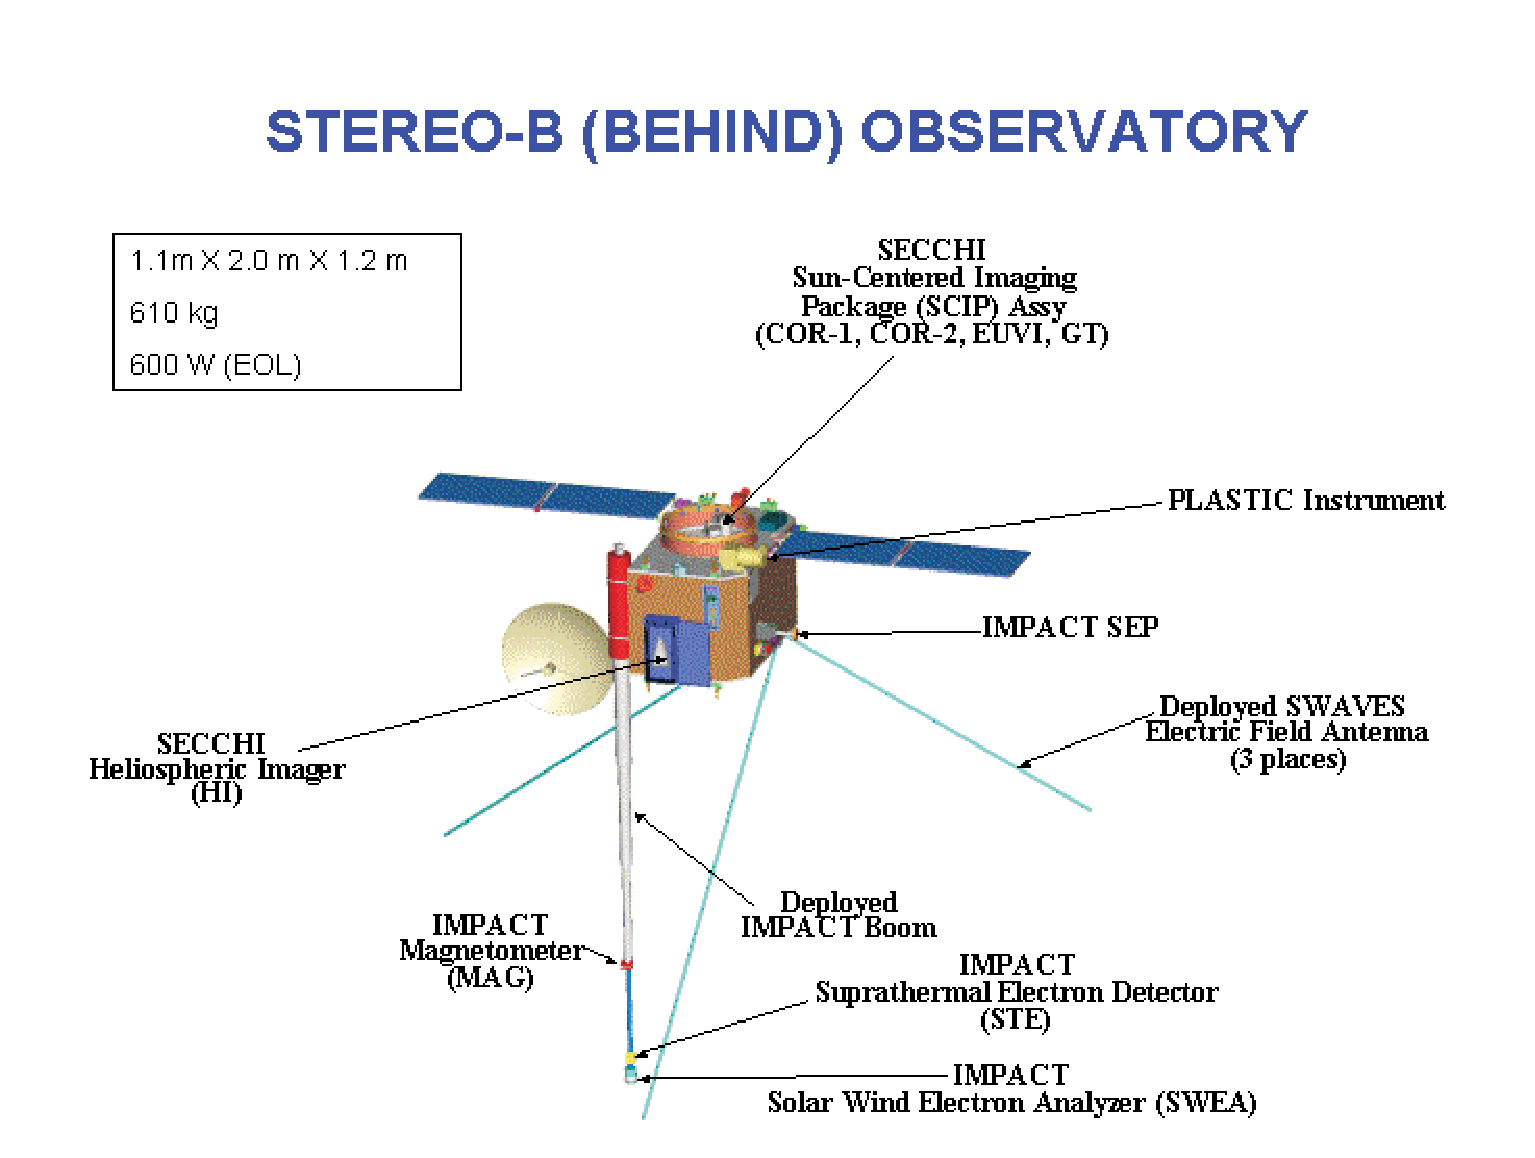
\includegraphics[width=20pc]{instruments.eps}
  \caption{Artist's view of STEREO B spacecraft, with permission of NASA}\label{fig_stereo}
  \end{figure}


\begin{figure}
\noindent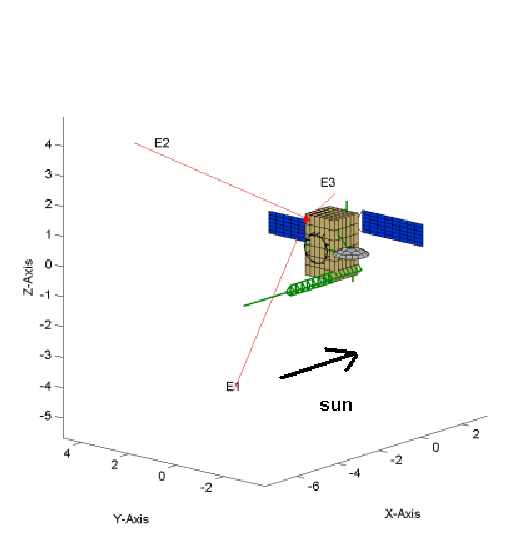
\includegraphics[width=20pc]{SpaceCraftD2HGA0Oblique.eps}
\caption{STEREO A}\label{fig_D2_A_Oblique}
 \end{figure}


 \begin{figure}
 \noindent 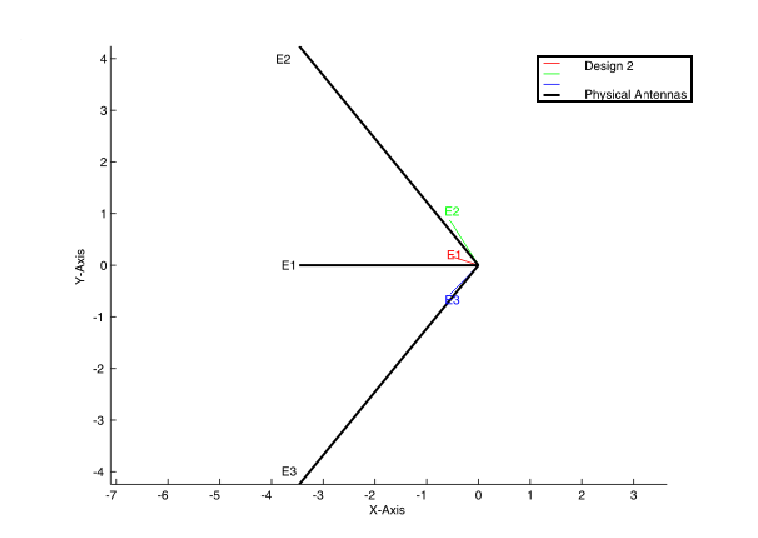
\includegraphics[width=20pc]{HeffD2HGA0-500kHz-ZViewCap.eps}
 \caption{STEREO A: Effective Length Vectors}\label{fig_Heff_D2_A_Z_ViewCap}
 \end{figure}


\begin{figure}
\noindent 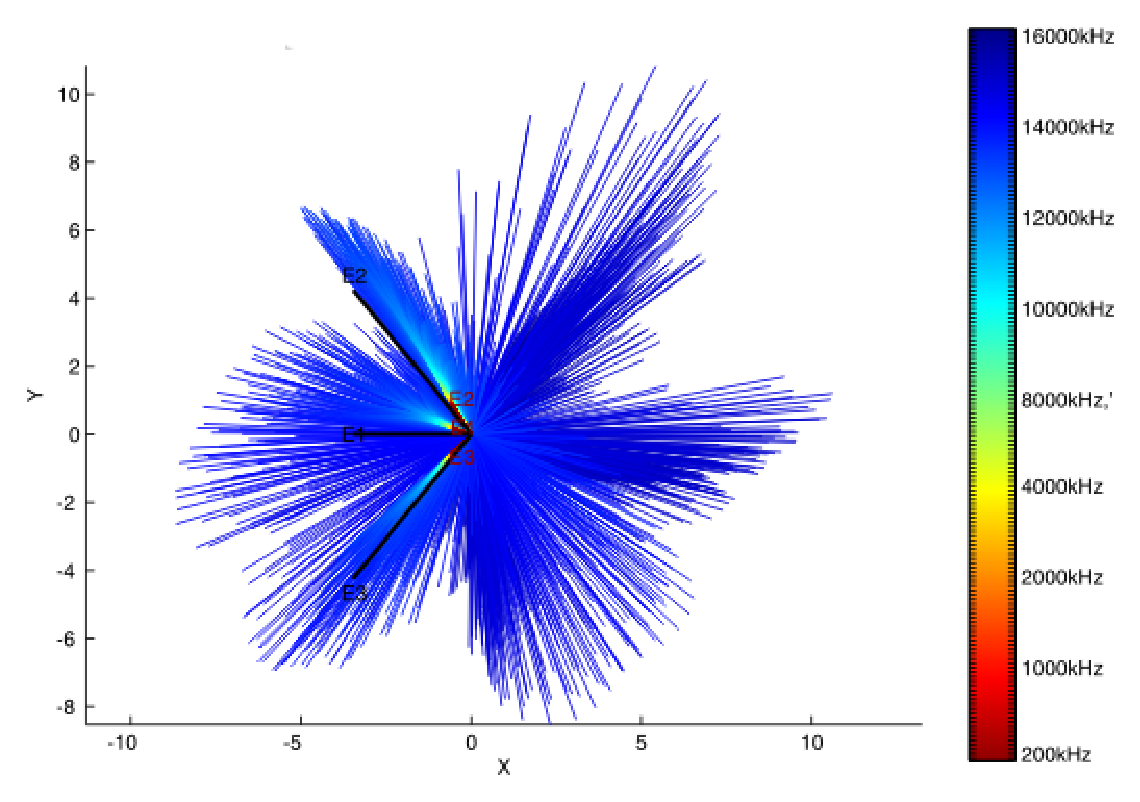
\includegraphics[width=20pc]{HeffVerteilungD2-ZView_caps.eps} \\
\caption{The spatial distribution of the real parts of the effective length vectors of STEREO A with a frequency up to 16MHz}\label{fig_heff_dist_D2_A_Z_View_caps}
\end{figure}

\begin{figure}
\noindent \includegraphics[width=20pc]{heff_length_variation500kHz_6d.eps} \\
\caption{The difference between the quasistatic effective length vector and the effective length vector in three dimensional complex space at 500kHz as function of direction of incidence.}\label{fig_heff_dist_6d_500kHz_caps}
\end{figure}

\begin{figure}
\noindent \includegraphics[width=20pc]{heff_length_variation13.5MHz_6d.eps} \\
\caption{The difference between the quasistatic effective length vector and the effective length vector in three dimensional complex space at 13.5MHz as function of direction of incidence.}\label{fig_heff_dist_6d_13.5MHz_caps}
\end{figure}



\begin{figure}
\noindent 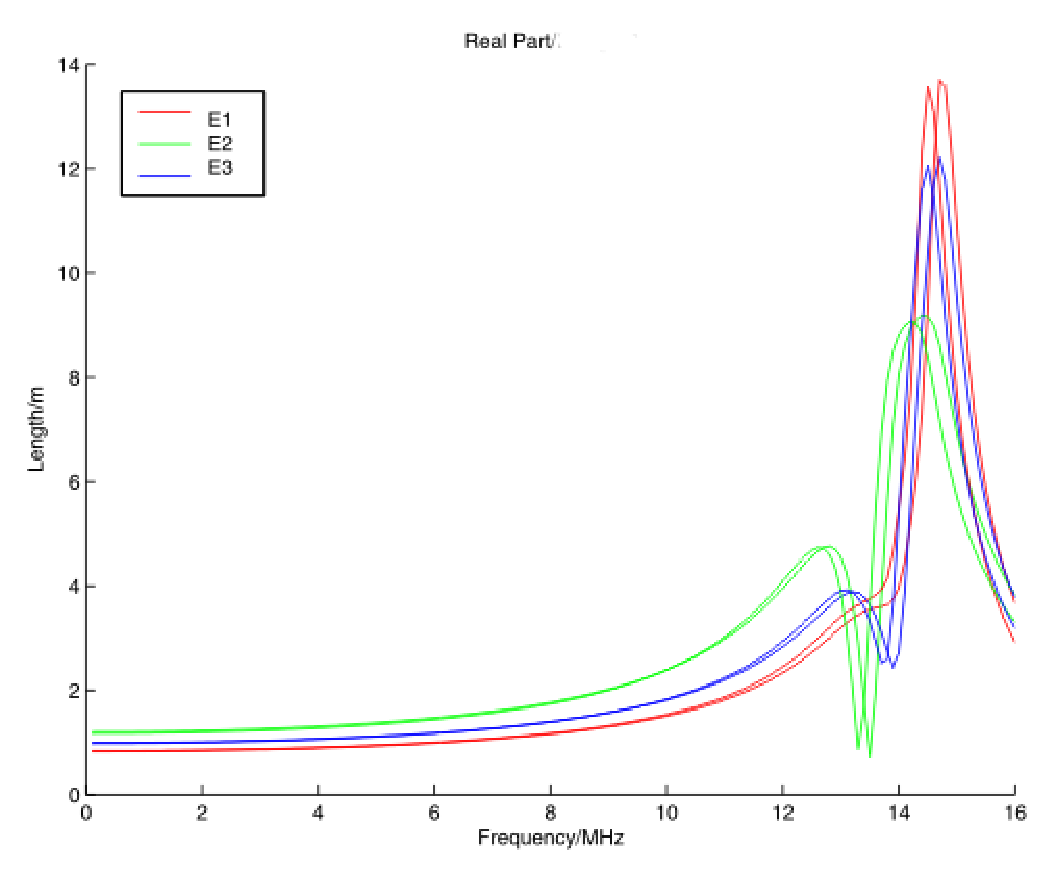
\includegraphics[width=20pc]{HeffLengthRealD2_caps.eps} \\
\caption{The length of the real parts of the electric antennas of STEREO A} \label{fig_Heff_length_real_caps_D2}
\end{figure}

\begin{figure}
\noindent 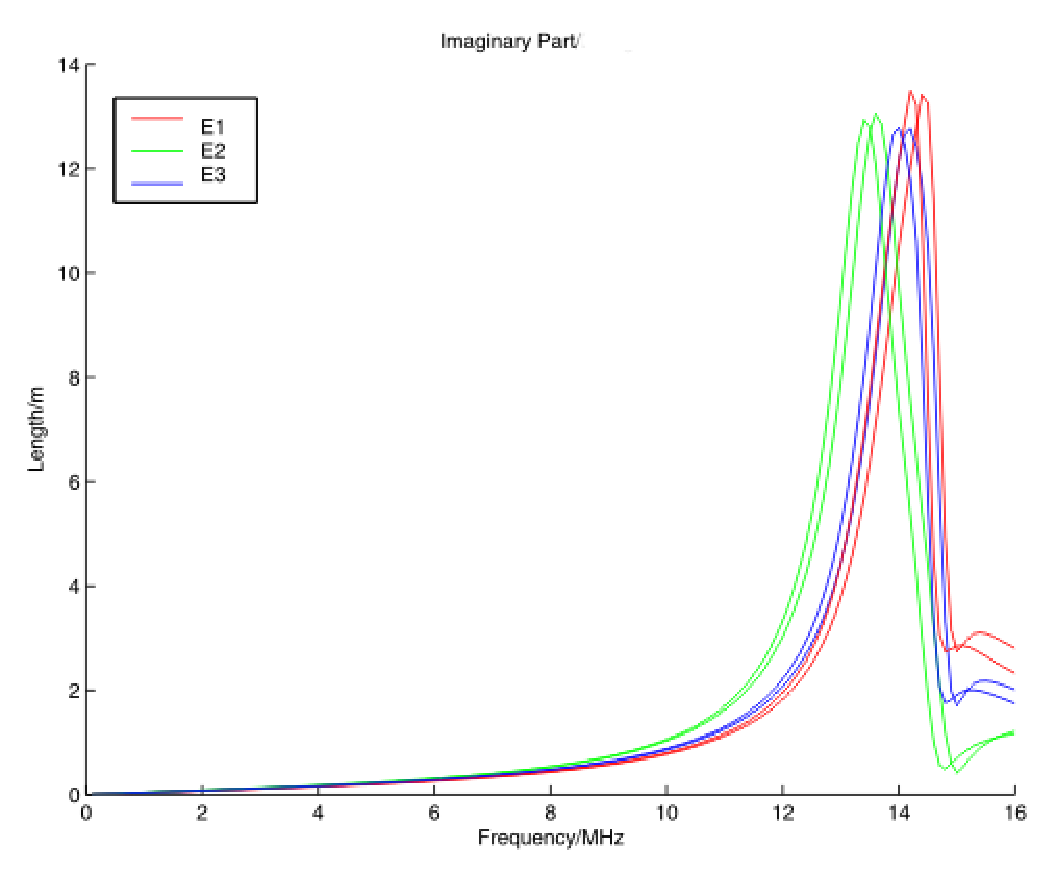
\includegraphics[width=20pc]{HeffLengthImagD2_caps.eps} \\
\caption{The length of the imaginary parts of the electric antennas of STEREO A} \label{fig_Heff_length_imag_caps_D2}
\end{figure}


 \begin{figure}
 \noindent 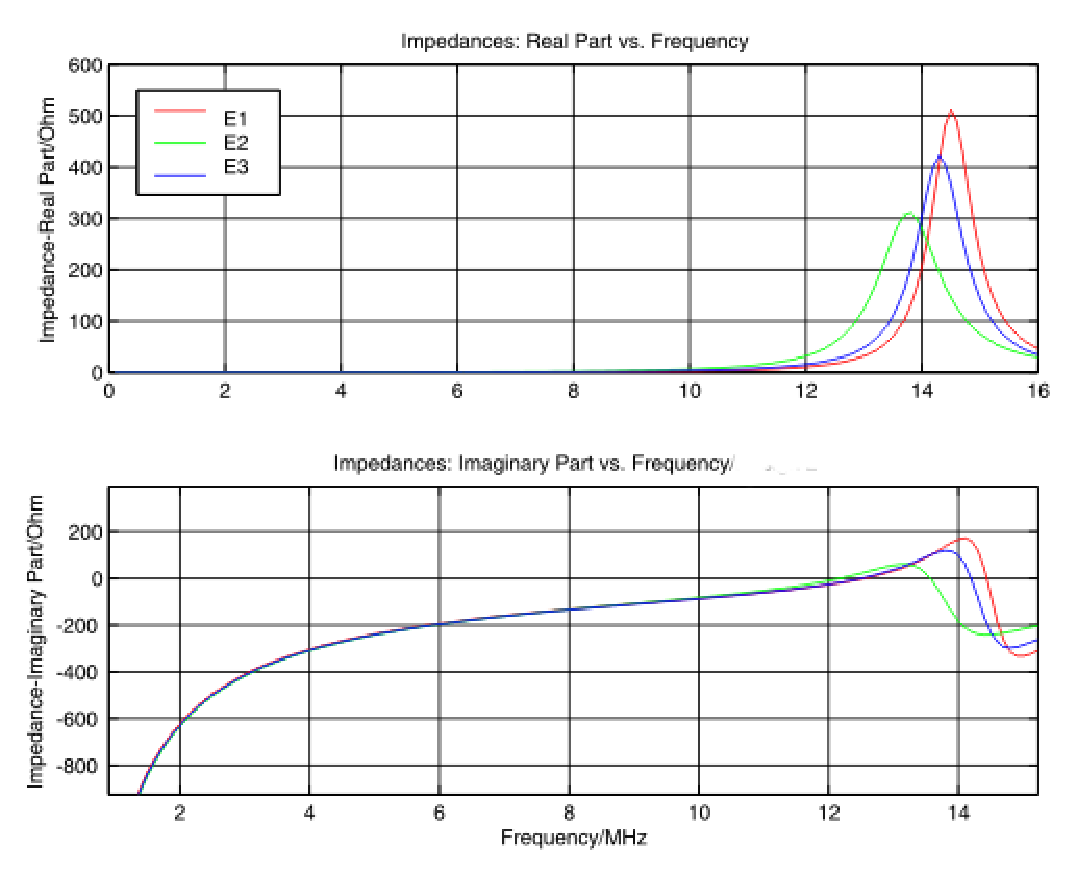
\includegraphics[width=20pc]{ImpedancesD21_caps.eps}\\ \caption{Impedances of STEREO A} \label{fig_Impedance1_D2_caps}
\end{figure}

\begin{figure}
\noindent 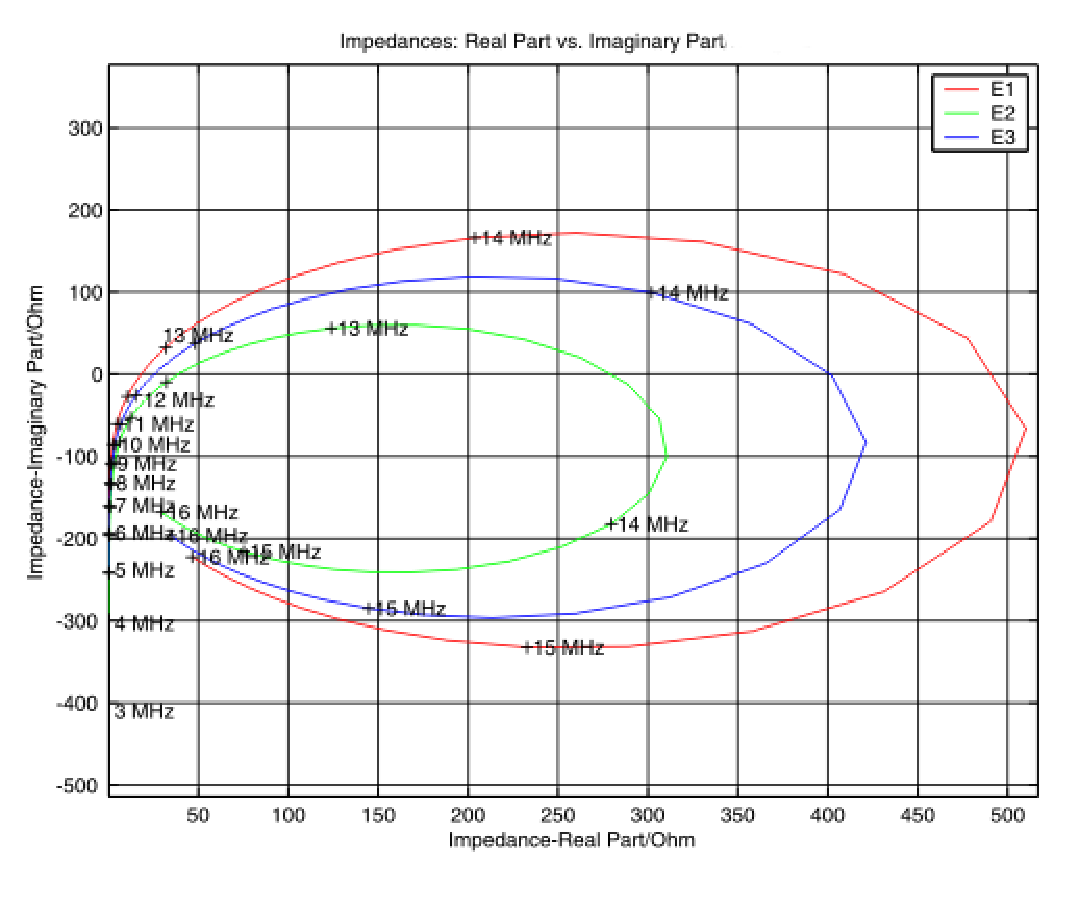
\includegraphics[width=20pc]{ImpedancesD22_caps.eps} \\ \caption{Impedances of STEREO A} \label{fig_Impedance2_D2_caps}
\end{figure}




\begin{table}  \label{tab_heff}
\caption{Effective length vectors at 500kHz}
\begin{flushleft}

\begin{tabular}{c|c|ccc}
\hline
&  & STEREO  & STEREO  & Physical  \\
& & A & B & antennas\\
\hline
 &Length/m& 0.83 &0.84&6.00\\
E1 & $\zeta/^\circ$ &128.3 & 127.2&125.26\\
 & $\xi/^\circ$ & 15.0& 13.3& 0.0\\
\hline
 &Length/m& 1.21 &1.18&6.00\\
E2 & $\zeta/^\circ$ &117.1 & 117.4&125.26\\
 & $\xi/^\circ$ & 125.8& 125.2& 120.0\\
\hline
 &Length/m& 0.99 &0.98&6.00\\
E3 & $\zeta/^\circ$ &123.5 & 123.3&125.26\\
 & $\xi/^\circ$ & -137.2& -135.4& -120.0\\
\hline
\end{tabular}
\end{flushleft}
\end{table}
%


\begin{table}
\caption{Variation of E1 due to HGA angle variation of STEREO A at 500kHz}\label{tab_e1_var}
\begin{flushleft}
\begin{tabular}{c|ccc}
\hline
HGA angle & $h_{eff}$ & $\zeta$ & $\xi$ \\
\hline
 -90 & 0.83 & 128.5 & 14.5 \\
 -80 & 0.83 & 128.5 & 14.5 \\
 -70 & 0.83 & 128.5 & 14.4 \\
 -60 & 0.83 & 128.4 & 14.5 \\
 -50 & 0.83 & 128.4 & 14.5 \\
 -40 & 0.83 & 128.4 & 14.5 \\
 -30 & 0.83 & 128.4 & 14.2 \\
 -20 & 0.83 & 128.3 & 14.7 \\
 -10 & 0.83 & 128.3 & 14.9 \\
 0 & 0.83 & 128.2 & 15.0 \\
 10 & 0.83 & 128.1 & 15.0 \\
 20 & 0.83 & 128.0 & 15.1 \\
 30 & 0.83 & 127.8 & 15.1 \\
 40 & 0.83 & 127.7 & 15.2 \\
 50 & 0.83 & 127.7 & 15.2 \\
 60 & 0.83 & 127.6 & 15.3 \\
 70 & 0.83 & 127.6 & 15.3 \\
 80 & 0.83 & 127.7 & 15.4 \\
 90 & 0.83 & 127.7 & 15.4 \\
\hline
\end{tabular}
\end{flushleft}
\end{table}



% \begin{figure}
% \noindent\includegraphics[width=20pc]{samplefigure.eps}
% \caption{Caption text here}
% \end{figure}
% \end{document}
%
% \begin{table}
% \caption{}
% \end{table}
%
% ---------------
% TWO-COLUMN figure/table
%
% \begin{figure*}
% \noindent\includegraphics[width=39pc]{samplefigure.eps}
% \caption{Caption text here}
% \end{figure*}
%
% \begin{table*}
% \caption{Caption text here}
% \end{table*}
%


% ---------------
% Landscape (broadside) figure/table
% (These objects will not display properly in draft mode, use galley.)
%
% ONE-COLUMN landscape figure and table
%
% \begin{landscapefigure}
% \includegraphics[height=.75\mycolumnwidth,width=42pc]{samplefigure.eps}
% \caption{Caption text here}
% \end{landscapefigure}
%
% \begin{landscapetable}
% \caption{Caption text here}
% \begin{tabular*}{\hsize}{@{\extracolsep{\fill}}lcccc}
% \tableline
% ....
% \tableline\\
% \multicolumn5l{(a) Algorithms from Numerical Recipes}\\
% \end{tabular*}
% \tablenotetext{}{}
% \tablecomments{}
% \end{landscapetable}
%
% FULL-PAGE landscape figures and tables
%
% \begin{figure*}[p]
% \begin{landscapefigure*}
% illustration here
% \caption{caption here}
% \end{landscapefigure*}
% \end{figure*}
%
% \begin{table}[p]
% \begin{landscapetable*}
% \caption{}
% \begin{tabular*}{\textheight}{@{\extracolsep{\fill}}lccrrrcrrr}
% ....
% \end{tabular*}
% \begin{tablenotes}
% ...
% \end{tablenotes}
% \end{landscapetable*}
% \end{table}
%

%% ------------------------------------------------------------------------ %%
%
%  END ARTICLE
%
%% ------------------------------------------------------------------------ %%

\end{article}



\end{document}
